%%%%%%%%%%%%%%%%%%%%%%%%%%%%%%%%%%%%%%%%%
% Programming/Coding Assignment
% LaTeX Template
%
% This template has been downloaded from:
% http://www.latextemplates.com
%
% Original author:
% Ted Pavlic (http://www.tedpavlic.com)
%
% Note:
% The \lipsum[#] commands throughout this template generate dummy text
% to fill the template out. These commands should all be removed when 
% writing assignment content.
%
% This template uses a Perl script as an example snippet of code, most other
% languages are also usable. Configure them in the "CODE INCLUSION 
% CONFIGURATION" section.
%
%%%%%%%%%%%%%%%%%%%%%%%%%%%%%%%%%%%%%%%%%

%----------------------------------------------------------------------------------------
%	PACKAGES AND OTHER DOCUMENT CONFIGURATIONS
%----------------------------------------------------------------------------------------

\documentclass{article}

\usepackage{fancyhdr} % Required for custom headers
\usepackage{lastpage} % Required to determine the last page for the footer
\usepackage{extramarks} % Required for headers and footers
\usepackage[usenames,dvipsnames]{color} % Required for custom colors
\usepackage{graphicx} % Required to insert images
\usepackage{listings} % Required for insertion of code
\usepackage{courier} % Required for the courier font
\usepackage{lipsum} % Used for inserting dummy 'Lorem ipsum' text into the template

\usepackage{float}
\usepackage{amsfonts}
\usepackage{amsmath}
\usepackage{bm}

% Margins
\topmargin=-0.45in
\evensidemargin=0in
\oddsidemargin=0in
\textwidth=6.5in
\textheight=9.0in
\headsep=0.25in

\linespread{1.1} % Line spacing

% Set up the header and footer
\pagestyle{fancy}
\lhead{K. Holmbeck and D. Tonne} % Top left header
\chead{\hmwkClass\ : \hmwkTitle} % Top center head
\rhead{\firstxmark} % Top right header
\lfoot{\lastxmark} % Bottom left footer
\cfoot{} % Bottom center footer
\rfoot{Page\ \thepage\ of\ \pageref{LastPage}} % Bottom right footer
\renewcommand\headrulewidth{0.4pt} % Size of the header rule
\renewcommand\footrulewidth{0.4pt} % Size of the footer rule

\setlength\parindent{0pt} % Removes all indentation from paragraphs

%----------------------------------------------------------------------------------------
%	CODE INCLUSION CONFIGURATION
%----------------------------------------------------------------------------------------

\usepackage{color} %red, green, blue, yellow, cyan, magenta, black, white
\definecolor{mygreen}{RGB}{28,172,0} % color values Red, Green, Blue
\definecolor{mylilas}{RGB}{170,55,241}

\lstset{language=Matlab,%
    basicstyle=\ttfamily\footnotesize,breaklines=true
    %basicstyle=\footnotesize\color{red},
    breaklines=true,%
    xleftmargin=0.5in,
    %xrightmargin=0.25in,
    morekeywords={matlab2tikz},
    keywordstyle=\color{blue},%
    morekeywords=[2]{1}, keywordstyle=[2]{\color{black}},
    identifierstyle=\color{black},%
    stringstyle=\color{mylilas},
    commentstyle=\color{mygreen},%
    showstringspaces=false,%without this there will be a symbol in the places where there is a space
    numbers=left,%
    numberstyle={\tiny \color{black}},% size of the numbers
    numbersep=9pt, % this defines how far the numbers are from the text
    emph=[1]{for,end,break},emphstyle=[1]\color{blue}, %some words to emphasise
    %emph=[2]{word1,word2}, emphstyle=[2]{style},    
}


%----------------------------------------------------------------------------------------
%	DOCUMENT STRUCTURE COMMANDS
%	Skip this unless you know what you're doing
%----------------------------------------------------------------------------------------

% Header and footer for when a page split occurs within a problem environment
\newcommand{\enterProblemHeader}[1]{
%\nobreak\extramarks{#1}{#1 continued on next page\ldots}\nobreak
%\nobreak\extramarks{#1 (continued)}{#1 continued on next page\ldots}\nobreak
}

% Header and footer for when a page split occurs between problem environments
\newcommand{\exitProblemHeader}[1]{
\nobreak\extramarks{#1 (continued)}{#1 continued on next page\ldots}\nobreak
\nobreak\extramarks{#1}{}\nobreak
}

\setcounter{secnumdepth}{0} % Removes default section numbers
\newcounter{homeworkProblemCounter} % Creates a counter to keep track of the number of problems

\newcommand{\homeworkProblemName}{}
\newenvironment{homeworkProblem}[1][Problem \arabic{homeworkProblemCounter}]{ % Makes a new environment called homeworkProblem which takes 1 argument (custom name) but the default is "Problem #"
\stepcounter{homeworkProblemCounter} % Increase counter for number of problems
\renewcommand{\homeworkProblemName}{#1} % Assign \homeworkProblemName the name of the problem
\subsection{\homeworkProblemName} % Make a section in the document with the custom problem count
\enterProblemHeader{\homeworkProblemName} % Header and footer within the environment
}{
\exitProblemHeader{\homeworkProblemName} % Header and footer after the environment
}

\newcommand{\problemAnswer}[1]{ % Defines the problem answer command with the content as the only argument
\noindent\framebox[\columnwidth][c]{\begin{minipage}{0.98\columnwidth}#1\end{minipage}} % Makes the box around the problem answer and puts the content inside
}

\newcommand{\homeworkSectionName}{}
\newenvironment{homeworkSection}[1]{ % New environment for sections within homework problems, takes 1 argument - the name of the section
\renewcommand{\homeworkSectionName}{#1} % Assign \homeworkSectionName to the name of the section from the environment argument
\subsection{\homeworkSectionName} % Make a subsection with the custom name of the subsection
\enterProblemHeader{\homeworkProblemName\ [\homeworkSectionName]} % Header and footer within the environment
}{
\enterProblemHeader{\homeworkProblemName} % Header and footer after the environment
}


%----------------------------------------------------------------------------------------
%   NAME AND CLASS SECTION
%----------------------------------------------------------------------------------------

\newcommand{\hmwkTitle}{Homework\ 4} % Assignment title
\newcommand{\hmwkDueDate}{Thursday,\ April\ 19,\ 2018} % Due date
\newcommand{\hmwkClass}{Math\ 521} % Course/clas
\newcommand{\hmwkAuthorName}{Kristin Holmbeck} % Your name

\DeclareMathOperator*{\argmax}{arg\,max}
\DeclareMathOperator*{\argmin}{arg\,min}

%----------------------------------------------------------------------------------------
%   TITLE PAGE
%----------------------------------------------------------------------------------------

\title{
\textmd{\textbf{\hmwkClass \ \hmwkTitle}}\\
\normalsize\vspace{0.1in}\small{Due\ on\ \hmwkDueDate}\\
\vspace{0.1in}
\vspace{0.2in}
}

\author{\textbf{\hmwkAuthorName}}
\date{} % Insert date here if you want it to appear below your name

%----------------------------------------------------------------------------------------

\begin{document}

\maketitle

%----------------------------------------------------------------------------------------
%   TABLE OF CONTENTS
%----------------------------------------------------------------------------------------

%\setcounter{tocdepth}{1} % Uncomment this line if you don't want subsections listed in the ToC
\vspace{0.75in}
\tableofcontents
\listoffigures
\newpage

%----------------------------------------------------------------------------------------
%   PROBLEM 1
%----------------------------------------------------------------------------------------

% To have just one problem per page, simply put a \clearpage after each problem

\begin{section}{Theory}

\begin{homeworkSection}{1. Eigen-relationship}

Consider the two eigenvector problems
\begin{align*}
	C_x \bm{u} = \lambda_x \bm{u}
\end{align*}
and
\begin{align*}
	C_s \bm{v} = \lambda_s \bm{v}
\end{align*}
where the matrices are related by $C_x = C_s + \alpha I$, where $\alpha$ is a real number and $I$ is the usual identity matrix. Show that if $\bm{u}$ is an eigenvector of $C_x$, then it is also an eigenvector of $C_s$ associated with eigenvalue $\lambda_s = \lambda_x -\alpha$.
\\
\\
\problemAnswer{
	\begin{align*}
		C_x \bm{u} &= \lambda_x \bm{u} = C_s \bm{u} + \alpha I \bm{u} \\
		C_s \bm{u} &= \lambda_x \bm{u} - \alpha I \bm{u} \\
		C_s \bm{u} &= (\lambda_x  - \alpha) \bm{u}  \\
		\text{but} \quad C_s \bm{v} &= \lambda_s \bm{v} \\
		\implies \lambda_s &= \lambda_x  - \alpha \qquad \text{is an eigenvalue of $C_s$ with associated eigenvector $\bm{u}$}
	\end{align*}
}

\end{homeworkSection}

\begin{homeworkSection}{2. Invertibility of a particular symmetric matrix}
Let $A \in \mathbb{R}^{m \times n}$. Show that the matrix $M$ defined as
\begin{align*}
	M &= \alpha^2 I + AA^T, \quad  \alpha \neq 0 \in \mathbb{R}
\end{align*}

is nonsingular, where $I = I_m$ and $\alpha$ is a nonzero real number.
\\
\\
\problemAnswer{
    First, we will show that $M$ is positive-definite.
    For any $x \neq 0 \in \mathbb{R}^m$,
    \begin{align*}
        x^T M x &= x^T (\alpha^2 I + AA^T) x = \alpha^2 x^T x + x^T AA^T x \\
                &= \alpha^2 ||x||^2 + ||A^T x||^2 \\
                &\geq \alpha^2 ||x||^2 \qquad \text{if $x \in$ null($A^T$)} > 0\\
        \implies x^T M x &> 0,
    \end{align*}
    thus, $M$ is positive definite which implies that the eigenvalues of $M$ are positive. Since zero cannot be an eigenvalue, $M$ is nonsingular.
    \\
}

\end{homeworkSection}

\begin{homeworkSection}{3. Between-Class Scatter Matrix simplification}
Show that the between-class scatter matrix, $S_B$, in the multi-class \textit{Fisher Discriminant Analysis} is given by
\begin{align*}
	S_B &= \sum_{i=1}^M n_i (\bm{m}_i - \bm{m})(\bm{m}_i - \bm{m})^T,
\end{align*}
where $M$ is the total number of distinct classes, $n_i$ is the number of data points in class $i$, $\bm{m}_i$ is the class mean of the $i^{\text{th}}$ class, and $m$ is the mean across all $n$ data points. You may use the facts that
\begin{align*}
	S_T = S_B + S_W, \quad S_W = \sum_{i=1}^M \sum_{x \in D_i} (x - \bm{m}_i)(x - \bm{m}_i)^T, \quad \text{and} \quad S_T = \sum_{i=1}^n (x_i - \bm{m})(x_i - \bm{m})^T
\end{align*}
\\
\\
\problemAnswer{
	Given what we know above, and the fact that the i$^{th}$ class mean $\bm{m}_i = \frac{1}{n_i} \sum_{x \in D_i} \bm{x}$ and the mean $\bm{m}$ across all data points is given by $\bm{m} = \frac{1}{n} \sum_{i=1}^n \bm{x}_i$, we will start with evaluating $S_B = S_T - S_W$.
	\\
	\\
	Furthermore, note that $\forall \bm{x}_i \in X$ (the entire data set), $\bm{x}_i \in \bigcup\limits_{j=1}^{M} D_j$, the union of all distinct classes, and also $\bm{m}_i n_i =  \sum_{x \in D_i} \bm{x}$.
	\\
	\begin{align*}
		S_T - S_W &= \sum_{i=1}^n (x_i - \bm{m})(x_i - \bm{m})^T - \sum_{i=1}^M \sum_{x \in D_i} (x - \bm{m}_i)(x - \bm{m}_i)^T \\
		&= \sum_{i=1}^M \sum_{x \in D_i} \left [ (x - \bm{m})(x - \bm{m})^T - (x - \bm{m}_i)(x - \bm{m}_i)^T \right ] \\
		&= \sum_{i=1}^M \sum_{x \in D_i} \left [ (x x^T - \bm{m} x^T -x \bm{m}^T + \bm{m}\bm{m}^T )- (xx^T - \bm{m}_i x^T - x {\bm{m}_i}^T + \bm{m}_i {\bm{m}_i}^T) \right ] \\
		&= \sum_{i=1}^M \sum_{x \in D_i} \left [ (\bm{m}\bm{m}^T - \bm{m} x^T -x \bm{m}^T )- (\bm{m}_i {\bm{m}_i}^T - \bm{m}_i x^T - x {\bm{m}_i}^T) \right ] \\
		&= \sum_{i=1}^M \left [ n_i \bm{m}\bm{m}^T - n_i \bm{m}_i {\bm{m}_i}^T + \sum_{x \in D_i}  (\bm{m}_i x^T + x {\bm{m}_i}^T - \bm{m} x^T - x \bm{m}^T ) \right ] \\
		&= \sum_{i=1}^M \left [ n_i \bm{m}\bm{m}^T - n_i \bm{m}_i {\bm{m}_i}^T + \bm{m}_i \sum_{x \in D_i} x^T + {\bm{m}_i}^T \sum_{x \in D_i} x - \bm{m} \sum_{x \in D_i} x^T - \bm{m}^T \sum_{x \in D_i} x \right ] \\
		&= \sum_{i=1}^M \left [ n_i \bm{m}\bm{m}^T - n_i \bm{m}_i {\bm{m}_i}^T + \bm{m}_i n_i {\bm{m}_i}^T + {\bm{m}_i}^T n_i {\bm{m}_i} - \bm{m} n_i {\bm{m}_i}^T - \bm{m}^T n_i {\bm{m}_i} \right ] \\
		&= \sum_{i=1}^M n_i \left [ \bm{m}\bm{m}^T + {\bm{m}_i}^T {\bm{m}_i} - \bm{m} {\bm{m}_i}^T - \bm{m}^T {\bm{m}_i} \right ] \\
		&= \sum_{i=1}^M n_i (\bm{m} - \bm{m}_i)(\bm{m} - \bm{m}_i)^T
		\\
	\end{align*}
}
\end{homeworkSection}

\end{section}

%----------------------------------------------------------------------------------------
\newpage

\begin{section}{Computing}

\begin{homeworkSection}{1. KL Procedure for Gappy Data}
This project concerns the application of the KL procedure for incomplete data \cite{everson}. Let the complete data set be translation-invariant:
\begin{align*}
	f(x_m, t_\mu) &= \frac{1}{N} \sum_{k=1}^N \frac{1}{k} \sin[k(x_m-  t_\mu)],
\end{align*}
where $m = 1,\ldots, M$, with $M$ dimension of the ambient space (size of the spatial grid), and $\mu = 1,\ldots,P$, with $P$ the number of points in the ensemble. 
\\
\\
Let $x_m = \cfrac{2\pi(m-1)}{M}$ and $t_\mu = \cfrac{2\pi(\mu-1)}{P}$.
\\
\\
Select an ensemble of masks $\lbrace \bm{m}^{(\mu)} \rbrace$, $\mu = 1, \ldots, P$. where 10\% of the indices are selected to be zero for each mask. Each pattern in the incomplete ensemble may be written as
\begin{align*}
	\tilde{\bm{x}}^{(\mu)} &= \bm{m}^{(\mu)} . \bm{f}^{(\mu)},
\end{align*}
where $\left ( \bm{f}^{(\mu)} \right )_m = \frac{1}{N} \sum_{k=1}^N \frac{1}{k} \sin[k(x_m-  t_\mu)]$. Let $P=M=64$ and $N=3$.

\renewcommand{\theenumi}{\alph{enumi}}
\begin{enumerate}
  \item Compute the eigenvectors of this ensemble using the gappy algorithm \cite{everson}.
  \item Plot the eigenvalues as a function of the iteration, and continue until they converge.
  \item Plot your final eigenfunctions corresponding to the 10 largest eigenvalues.
  \item Plot the element $\tilde{\bm{x}}^{(1)}$ and the vector $\tilde{\bm{x}}_D$ repaired 	according to Equation
  \begin{align}
  	\tilde{\bm{x}} \approx \tilde{\bm{x}}_D = \sum_{n=1}^D \tilde{a}_n \phi^{(n)}.
  \end{align}
  Determine the value of $D$ that provides the best approximation to the original non-gappy pattern vector.
\end{enumerate}

\problemAnswer{
    We begin by visualizing the true and gappy data (generated using a random mask) shown in Figures \ref{fig:true_data} and \ref{fig:gappy_data}, respectively.

    \begin{minipage}{0.5\textwidth}
        \begin{figure}[H]
        \centering
        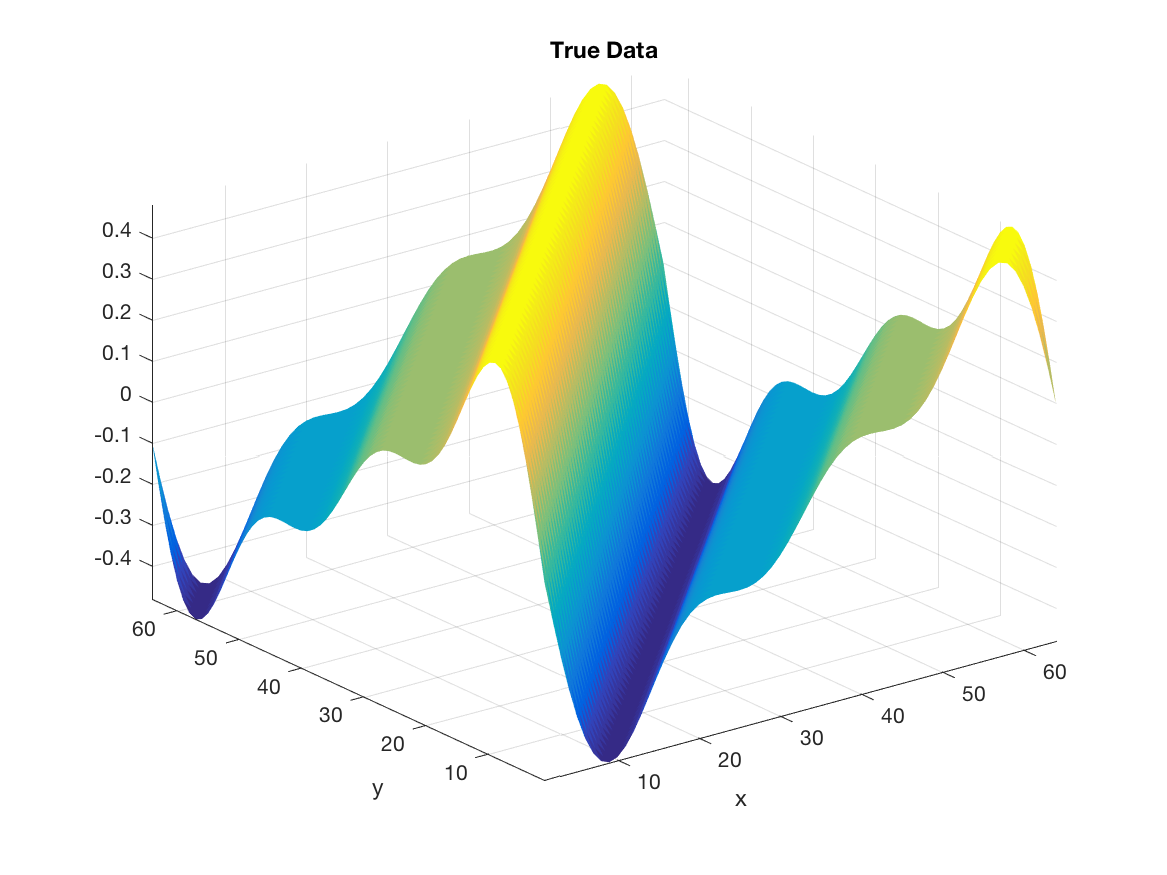
\includegraphics[trim={0cm 0cm 0cm 0cm},clip,width=1.0\columnwidth]{../data/true_data}
        \caption{True Data (Generated)}
        \label{fig:true_data}
        \end{figure}
    \end{minipage}
    \begin{minipage}{0.5\textwidth}
        \begin{figure}[H]
        \centering
        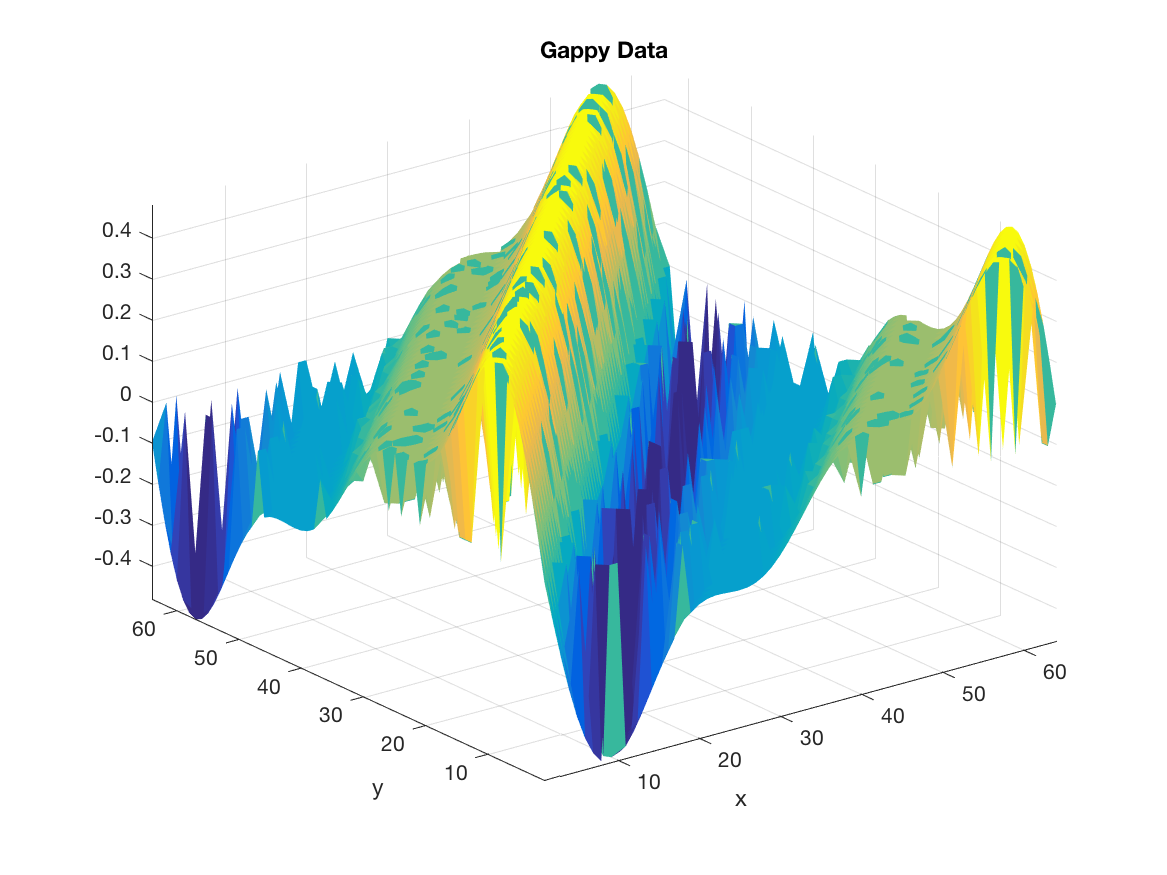
\includegraphics[trim={0cm 0cm 0cm 0cm},clip,width=1.0\columnwidth]{../data/gappy_data}
        \caption{Gappy Data (``Given")}
        \label{fig:gappy_data}
        \end{figure}
    \end{minipage}
}
\problemAnswer{
    The procedure for filling in the gappy data is outlined in \cite{chang}, and the actual code for doing so is given later in this document. Given a set of data $\lbrace \bm{x}^{(\mu)} \rbrace_{\mu=1}^P$ with each $\bm{x}^{(\mu)} \in \mathbb{R}^{M \times P}$, we initialize masks for each data point $\lbrace \bm{m}^{(\mu)} \rbrace_{\mu=1}^P$ to define our gappy data. If $m^{(\mu)}_i = 0$, there is a gap and we need to repair the data; if $m^{(\mu)}_i=1$, do nothing. We are changing/repairing only the gaps (defined by the 0-values in a mask vector $m$) with a \textit{repair} $\bm{r}$, where
    $$
        \bm{r} = \sum_{n=1}^D b_n U^{(n)}
    $$
    where $D$ is a rank-approximation value, and $\lbrace U^{(n)} \rbrace$ is a set of basis vectors (eigenvectors) of the data set $\lbrace x^{(\mu)} \rbrace_{\mu=1}^P$. The coefficients $b_n$ for each set of data are found by solving the system of equations
    $$
        \begin{bmatrix} \langle \bm{x}^{(\mu)}, U^{(1)} \rangle_m \\
        \vdots \\
        \langle \bm{x}^{(\mu)}, U^{(D)} \rangle_m
        \end{bmatrix}
        =
        \begin{bmatrix}
            \langle U^{(1)}, U^{(1)} \rangle_m && \cdots && \langle U^{(1)}, U^{(D)} \rangle_m \\
            \vdots && \ddots && \vdots \\
            \langle U^{(D)}, U^{(1)} \rangle_m && \cdots && \langle U^{(D)}, U^{(D)} \rangle_m \\
        \end{bmatrix}
        \begin{bmatrix} b_1 \\ \vdots \\ b_D \end{bmatrix}        
    $$
    where $\langle U^{(i)}, U^{(j)} \rangle_{\bm{m}}$ is the dot product of $U^{(i)}, U^{(j)}$ with the applied mask $\bm{m}$. In other words,
    $$
        \langle U^{(i)}, U^{(j)} \rangle_{\bm{m}} = 
        \begin{bmatrix}
            U^{(i)}_1 m_1 && U^{(i)}_2 m_2 && \cdots && U^{(i)}_M m_M
        \end{bmatrix}
        \begin{bmatrix}
            U^{(j)}_1 m_1 \\ U^{(j)}_2 m_2 \\\vdots \\ U^{(j)}_M m_M
        \end{bmatrix}
    $$
    Solving for the repair $\bm{r}$ for each $\bm{x}^{(\mu)}$ gives us an approximation to the true data set, and we iterate this algorithm until convergence. With that, let's look at the results for the data set shown in Figure \ref{fig:true_data}. We use the first iteration of this algorithm to determine an appropriate $D$-approximation to the data set.
    \begin{minipage}{1.0\textwidth}
        \begin{figure}[H]
        \centering
        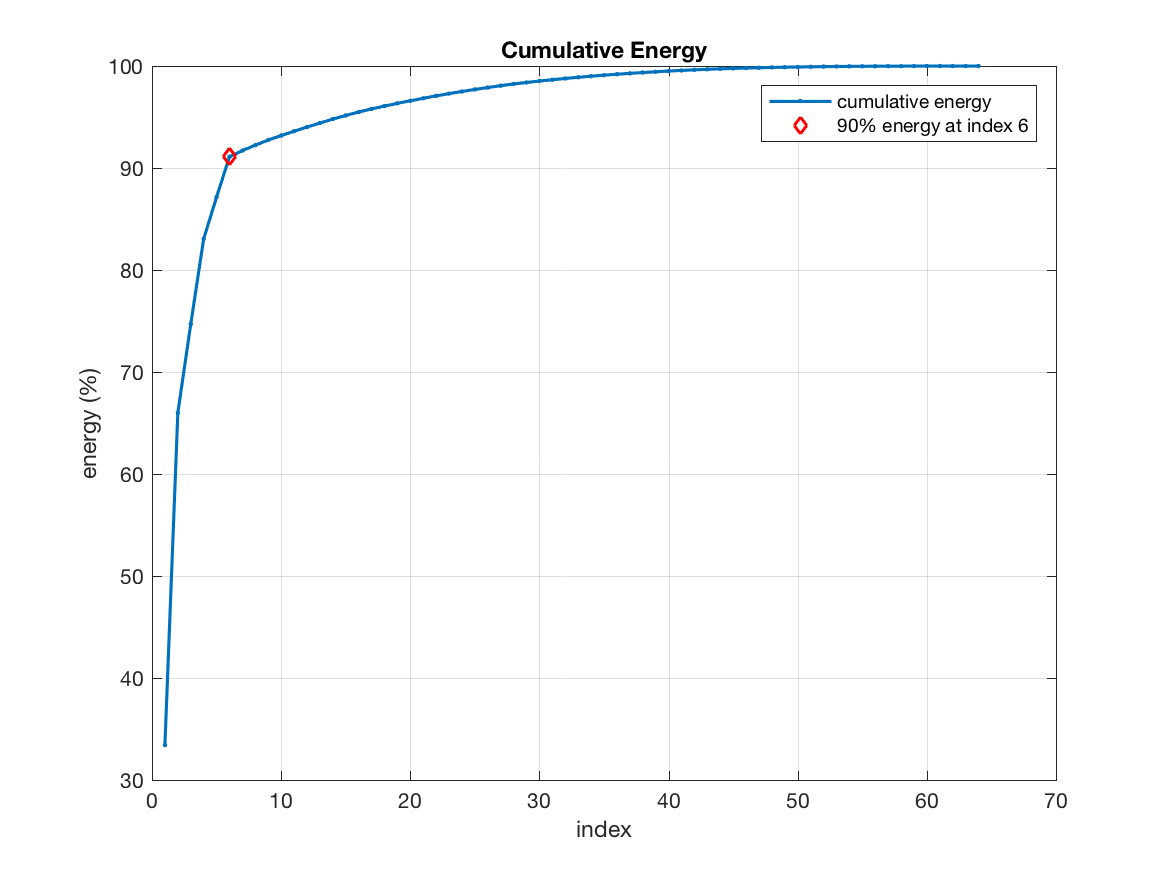
\includegraphics[trim={0cm 0cm 0cm 0cm},clip,width=0.70\columnwidth]{../data/cumulative_energy}
        \caption{Cumulative energy of the mean-subtracted gappy data}
        \label{fig:energy}
        \end{figure}
    \end{minipage}
}
\newpage
\problemAnswer{
    From Figure \ref{fig:energy}, we select a $D=6$ rank approximation of the data to retain 90\% of the energy. So for the remaining iterations, we will use the rank-6 approximation when obtaining the best basis (SVD). To further illustrate this point, we plot the first gappy data point along with its repair, i.e. estimation of the gappy data using the coefficients $b_n$ from above:
    \\
    \begin{minipage}{1.0\textwidth}
        \begin{figure}[H]
        \centering
        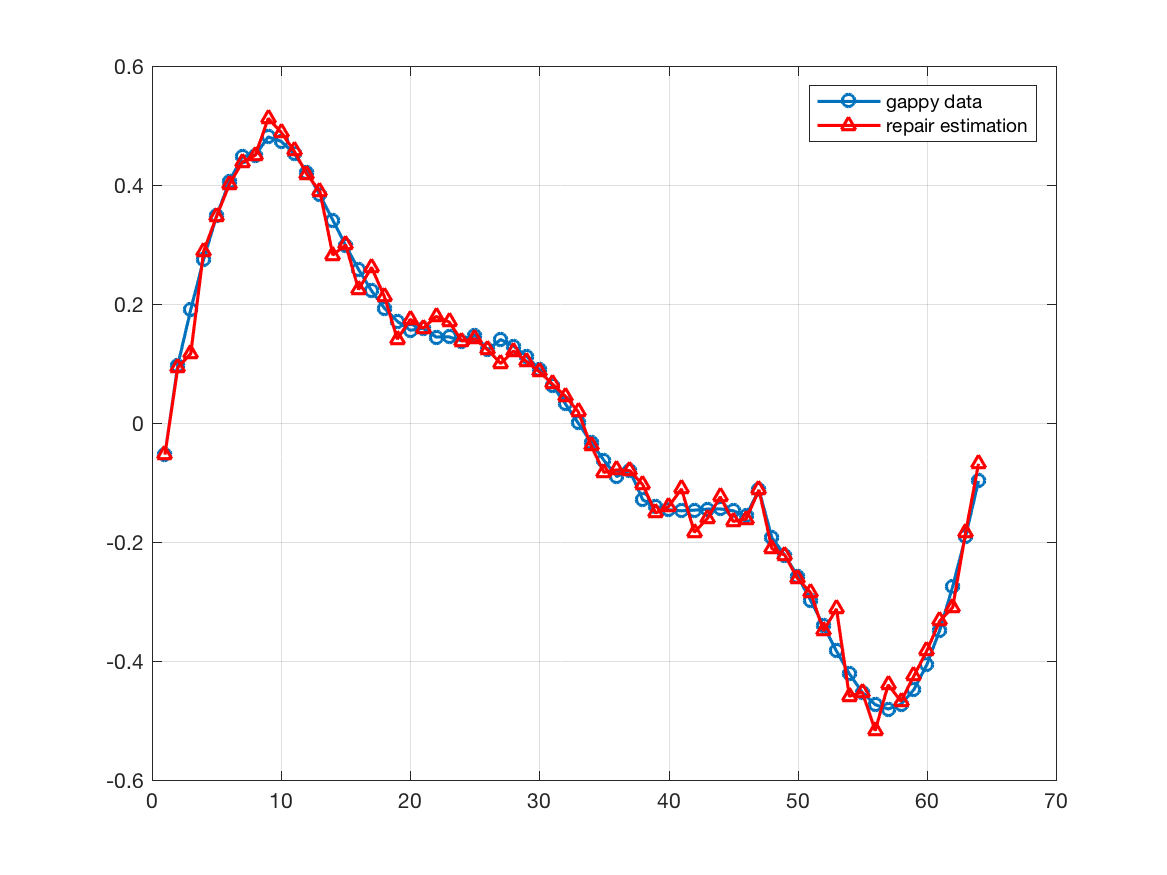
\includegraphics[trim={0cm 1cm 0cm 1cm},clip,width=0.70\columnwidth]{../data/x1}
        \caption{First iteration repair}
        \label{fig:x1}
        \end{figure}
    \end{minipage}
    \\
    \\
    \\
    Using this rank-6 approximation, we iterate until convergence using the eigenvalues of the repaired data as a critera: when the maximum absolute change in eigenvalues falls below $1e-4$, we consider the algorithm to have converged. With this tolerance, the algorithm converges in 8 iterations. For a tolerance of $1e-8$, we get convergence in 18 iterations. The convergence of the eigenvalues is shown in Figure \ref{fig:eigval_convergence}.
    \\
    \begin{minipage}{1.0\textwidth}
        \begin{figure}[H]
        \centering
        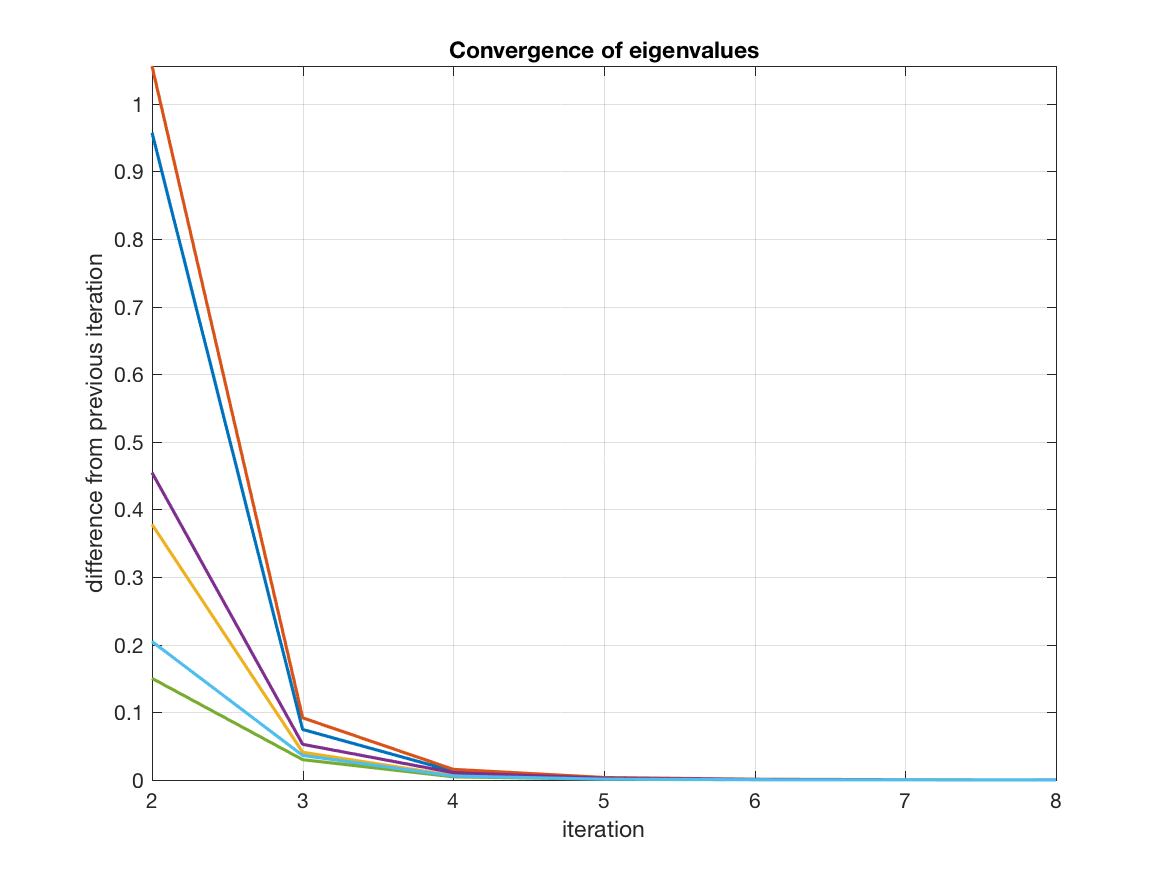
\includegraphics[trim={0cm 1cm 0cm 0cm},clip,width=0.70\columnwidth]{../data/eigval_convergence}
        \caption{Eigenvalue convergence}
        \label{fig:eigval_convergence}
        \end{figure}
    \end{minipage}
}
\newpage
\problemAnswer{
   The convergence of the data is shown below with the error from the true data. Depending on the application, the repair given in iteration 3 is visually very similar to the true data from Figure \ref{fig:true_data}.
    \begin{minipage}{1.0\textwidth}
        \begin{figure}[H]
        \centering
        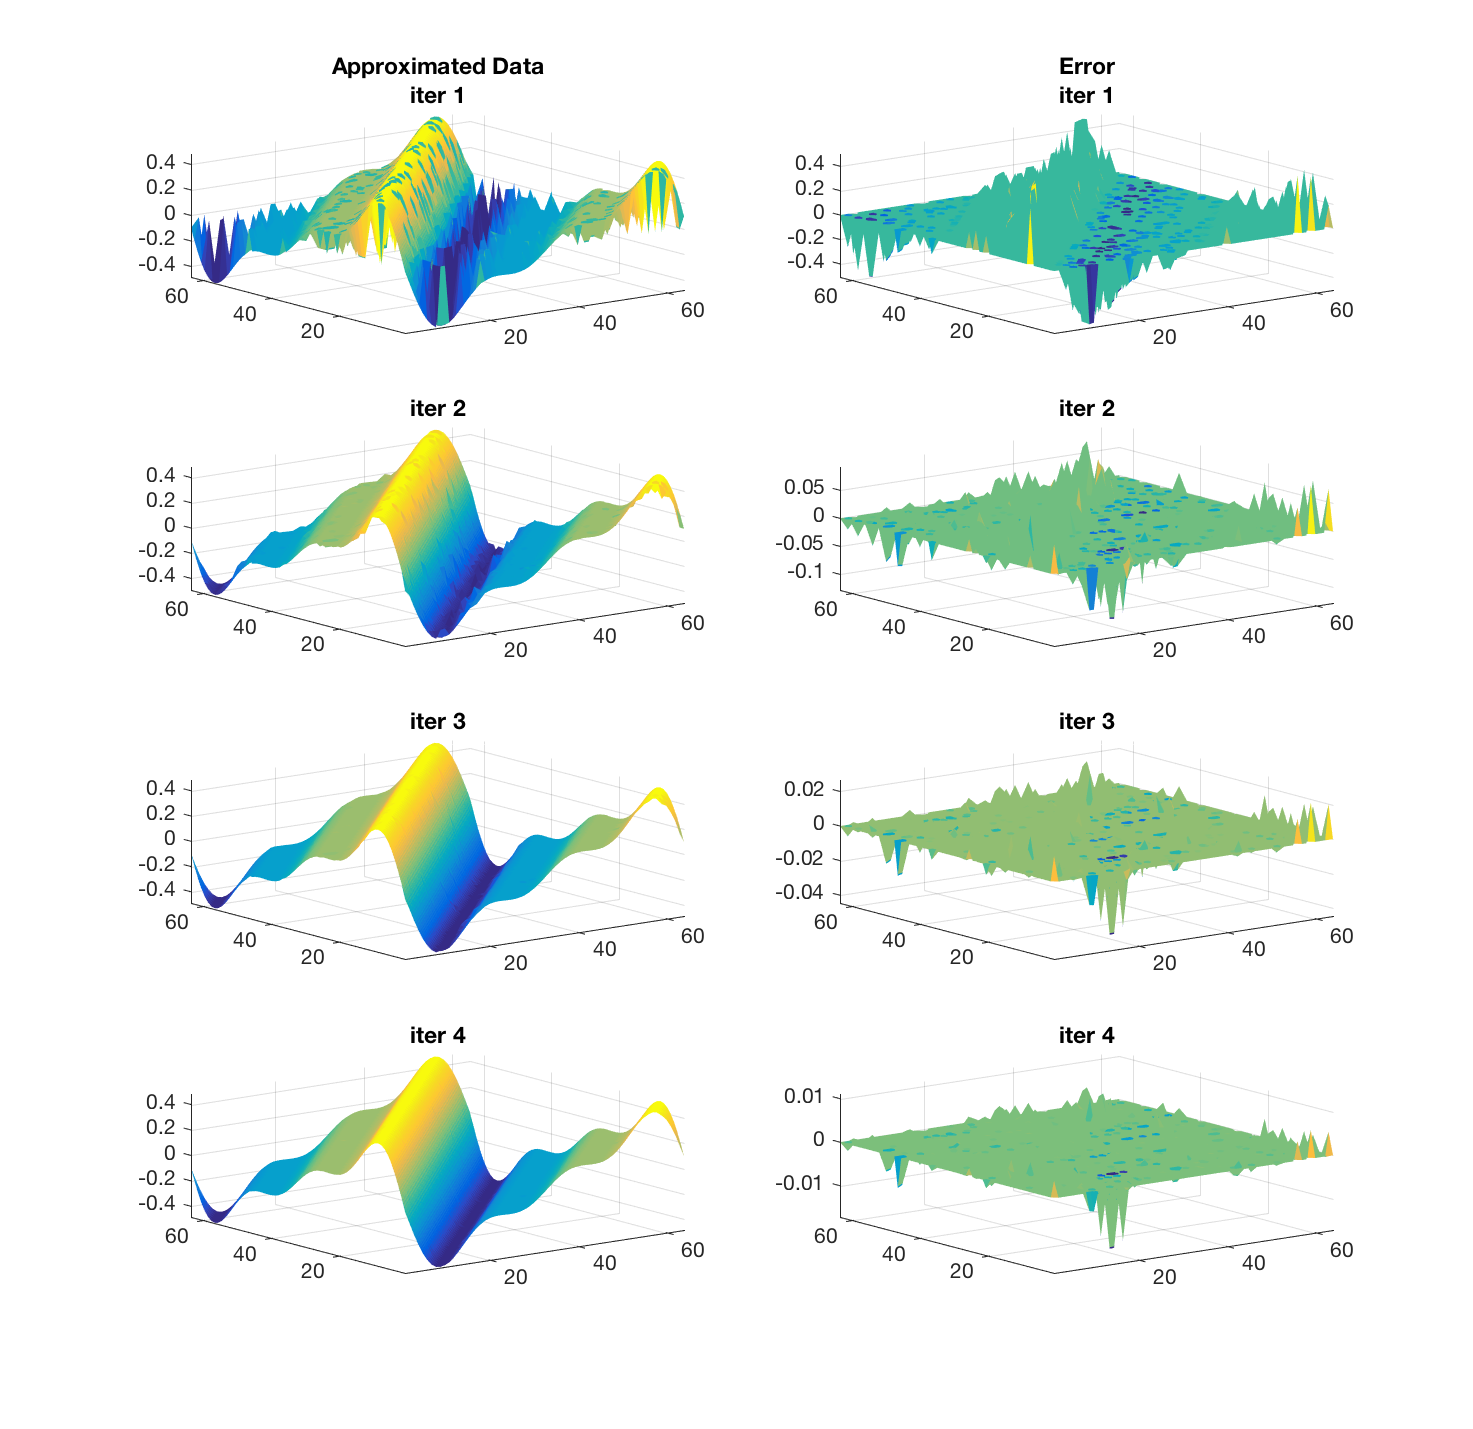
\includegraphics[trim={1cm 2cm 1cm 0cm},clip,width=0.90\columnwidth]{../data/data_convergence}
        \caption{Data convergence for the first 4 iterations}
        \label{fig:data_convergence}
        \end{figure}
    \end{minipage}
    \\
    \\
}
\problemAnswer{
    Let us also examine the first ten eigenvectors of the repaired set. As expected, the eigenvectors / eigenfunctions of this data are sinusoidal. Further eigenvectors do not show anything intuitive as they are associate with low singular values. For reference, the first several singular values are given as: 
    $\lbrace \frac{32}{3},\frac{32}{3},\frac{16}{3},\frac{16}{3},\frac{32}{9},\frac{32}{9},
    0.0006,
    0.0002,
    0.0002,
    0.0001,
    0.0001,
    0.0001 \rbrace$. As we can see, the first 6 eigenvalue-eigenvector pairs make up the bulk of the data. 
    \\
    \\
    \begin{minipage}{1.0\textwidth}
        \begin{figure}[H]
        \centering
        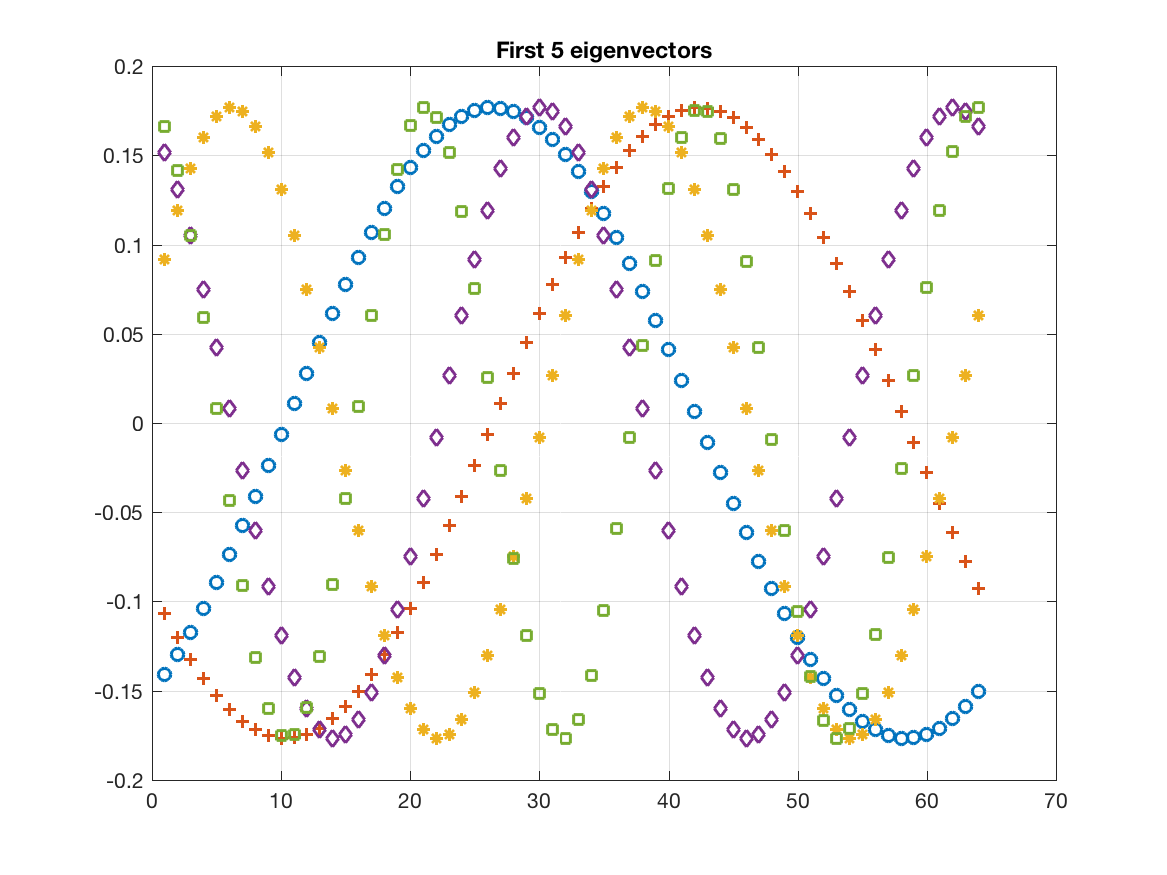
\includegraphics[trim={0cm 0cm 0cm 0cm},clip,width=0.60\columnwidth]{../data/eigvec_1}
        \caption{Eigenvectors 1 to 5}
        \label{fig:eigvec_1}
        \end{figure}
    \end{minipage}
    \begin{minipage}{1.0\textwidth}
        \begin{figure}[H]
        \centering
        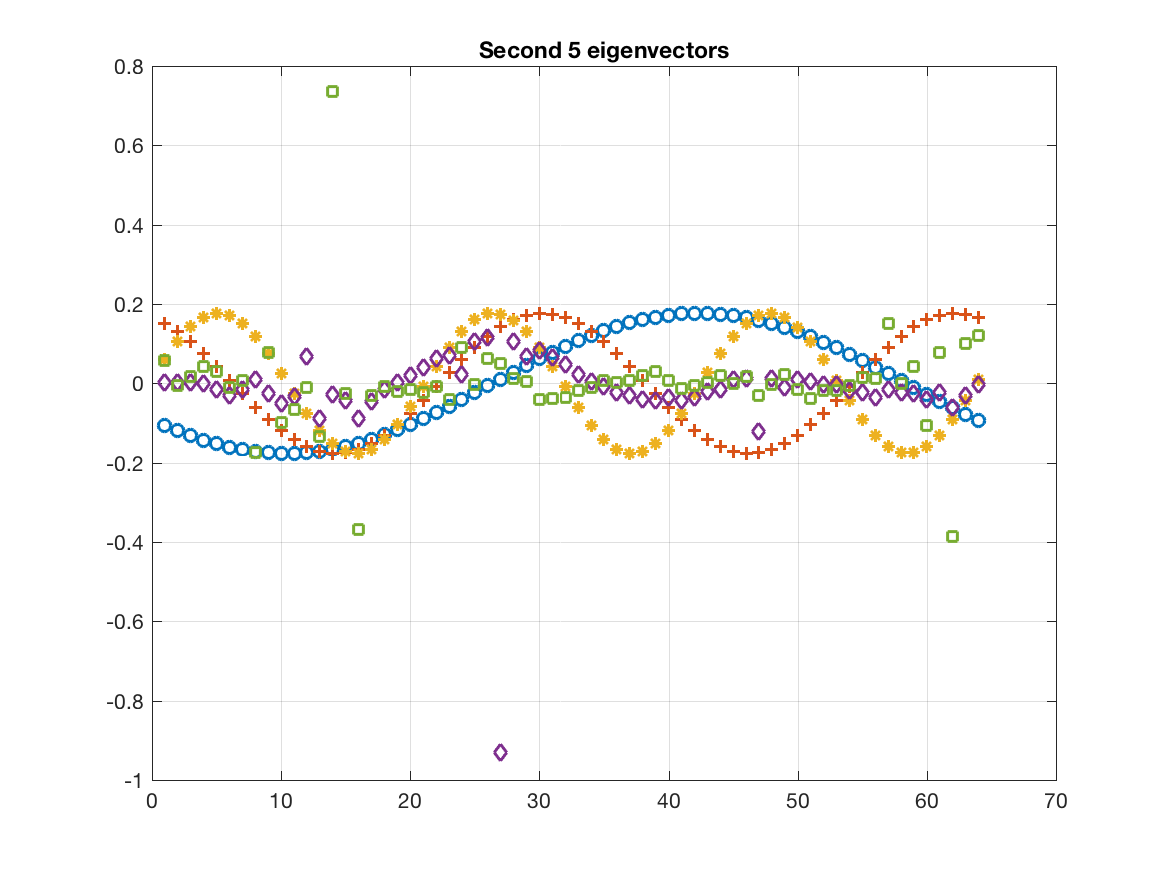
\includegraphics[trim={0cm 0cm 0cm 0cm},clip,width=0.60\columnwidth]{../data/eigvec_2}
        \caption{Eigenvectors 6 to 10}
        \label{fig:eigvec_2}
        \end{figure}
    \end{minipage}
    \\
    \\
}
\end{homeworkSection}

\newpage
\begin{homeworkSection}{2. Linear Discriminant Analysis (LDA)}
\renewcommand{\theenumi}{\alph{enumi}}
\begin{enumerate}
  \item Write a \textsc{MATLAB} routine to produce an optimal projection direction, $w$, using the two-class LDA
    criterion
    $$
        w = \argmax_w J(w) = \argmax_w \frac{w^T S_B w}{w^T S_W w},
    $$
    where
    $$
        S_B = (\bm{m}_2 - \bm{m}_1)(\bm{m}_2 - \bm{m}_1)^T \quad \text{and} \quad
        S_W = \sum_{i=1}^M \sum_{x \in D_i} (x - \bm{m}_i)(x - \bm{m}_i)^T
    $$
    are the between-class scatter matrix and the within-class scatter matrix, respectively. That is, your
    code should take in a set of data points with a clear indication which points belong to class 1 and
    which points belong to class 2, and output a single vector $w$ that is the solution of the generalized
    eigenvalue problem $S_B w = \lambda S_W w$.
  \item Now, use your subroutine in part (a) to project the EEG data onto a real line. Particularly, we can
    form a data point in $\mathbb{R}^{1040 \times 19}$ by concatenating the columns for each trial, therefore having 10 data
    points for task 2 and 10 data points for task 3. You would then project these 20 points onto the
    real line with the $w$ found with part (a). Plot the projected data on the real line and distinguish the
    classes with different symbols. Do you see a clear separation? Analyze your results.
\end{enumerate}

\problemAnswer{
    For the algorithm to make sense, we need to recall some important properties about the SVD. A data set (matrix) $X \in \mathbb{R}^{m \times p}$ ($m>p$, rank$(X)=p$) can be decomposed into the ``thin" SVD:
    $$
        X = U \Sigma V^T \implies U^T X = \Sigma V^T
    $$
    where $U$ is $m \times p$, $S$ is $p \times p$, and $V$ is $p \times p$. In our particular data, we have $X$ as an $19760 \times 20$ matrix, and it is not feasible to find the $S_B$ and $S_W$ matrices due to limited computer memory. If we instead perform LDA on $\tilde{X} = \Sigma V^T \in \mathbb{R}^{p \times p}$, we can use the projection vector $w$ on $\tilde{X}$ to classify the data. The code is include later in this document, but the general outline is this:
    \begin{itemize}
        \item Perform thin SVD on $X$: $[U,S,V]$ = svd$(X,0)$
        \item Apply PCA to obtain a $D$-rank approximation. We now have $\hat{U}, \hat{S}, \hat{V}$ that have $D$ columns each (instead of $p$ columns).
        \item Form a modified data set, $A = \hat{S} \hat{V}^T$ \cite{debbie}
        \item Formulate the between-class scatter matrix, $S_B$, and the within-class scatter matrix, $S_W$, based on $A$
        \item Get the eigenvector $w$ associated with the maximum eigenvalue of $S_W^{-1}S_B$
        \item Project: $w^T A$. This should give the desired classes.
    \end{itemize}
    The results for the EEG data shows clear separation, along with an interesting variation depending on how we calculate the SVD. In particular, we find that the separation is very clear when using just the SVD on $X$ to reduce the data (Figure \ref{fig:lda_1}). If we instead use SVD on $X - \langle X \rangle$, the mean-subtracted data, we obtain the results shown in Figure \ref{fig:lda_2}. There is still a clear separation between classes, and the data points are classified correctly, but the projected points have more variance in the $w$ space.
    \\
    \\
    As a quick guess, this may happen because the raw data has very strong variance between the classes. Performing SVD on the mean-subtracted \textit{entire} data set, we are normalizing both classes to be ``closer" together.
}
\problemAnswer{
    \begin{minipage}{1.0\textwidth}
        \begin{figure}[H]
        \centering
        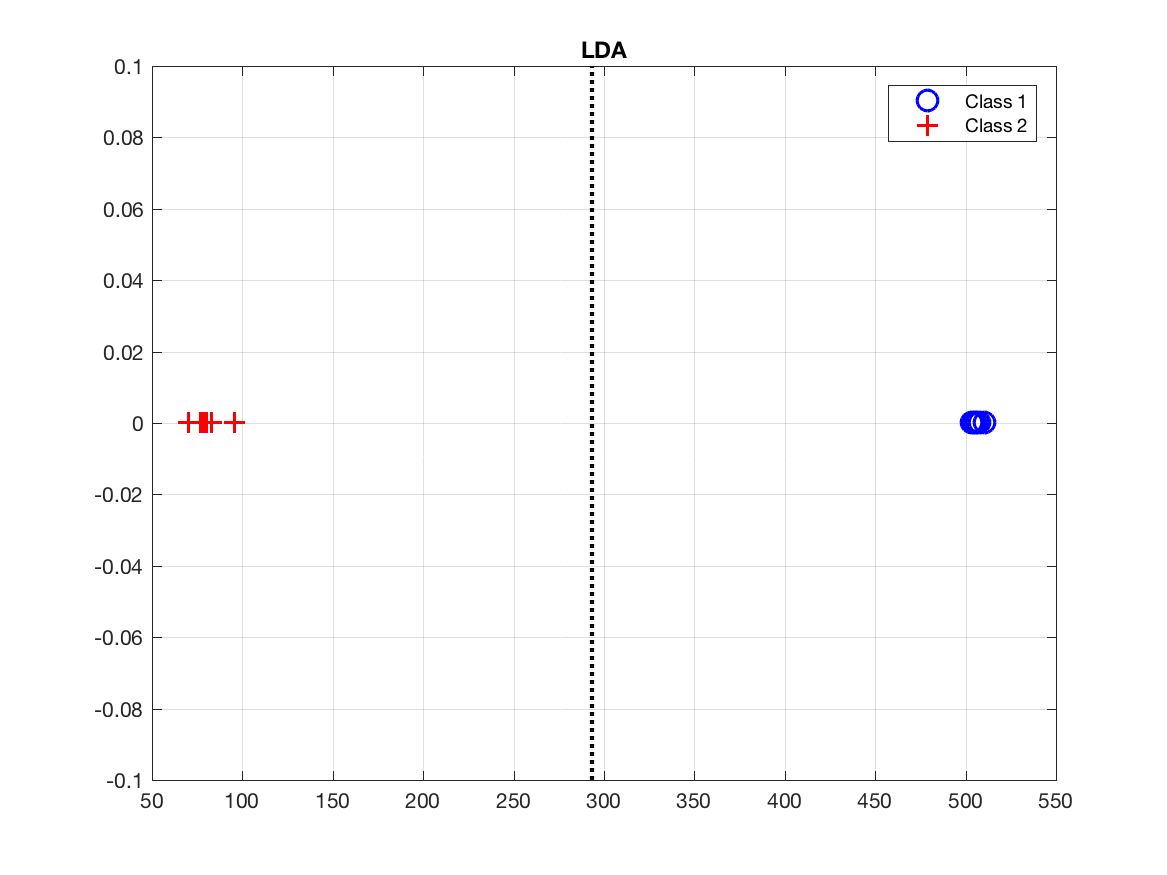
\includegraphics[trim={0cm 1cm 0cm 0cm},clip,width=0.60\columnwidth]{../data/classify}
        \caption{LDA using SVD directly}
        \label{fig:lda_1}
        \end{figure}
    \end{minipage}
    \begin{minipage}{1.0\textwidth}
        \begin{figure}[H]
        \centering
        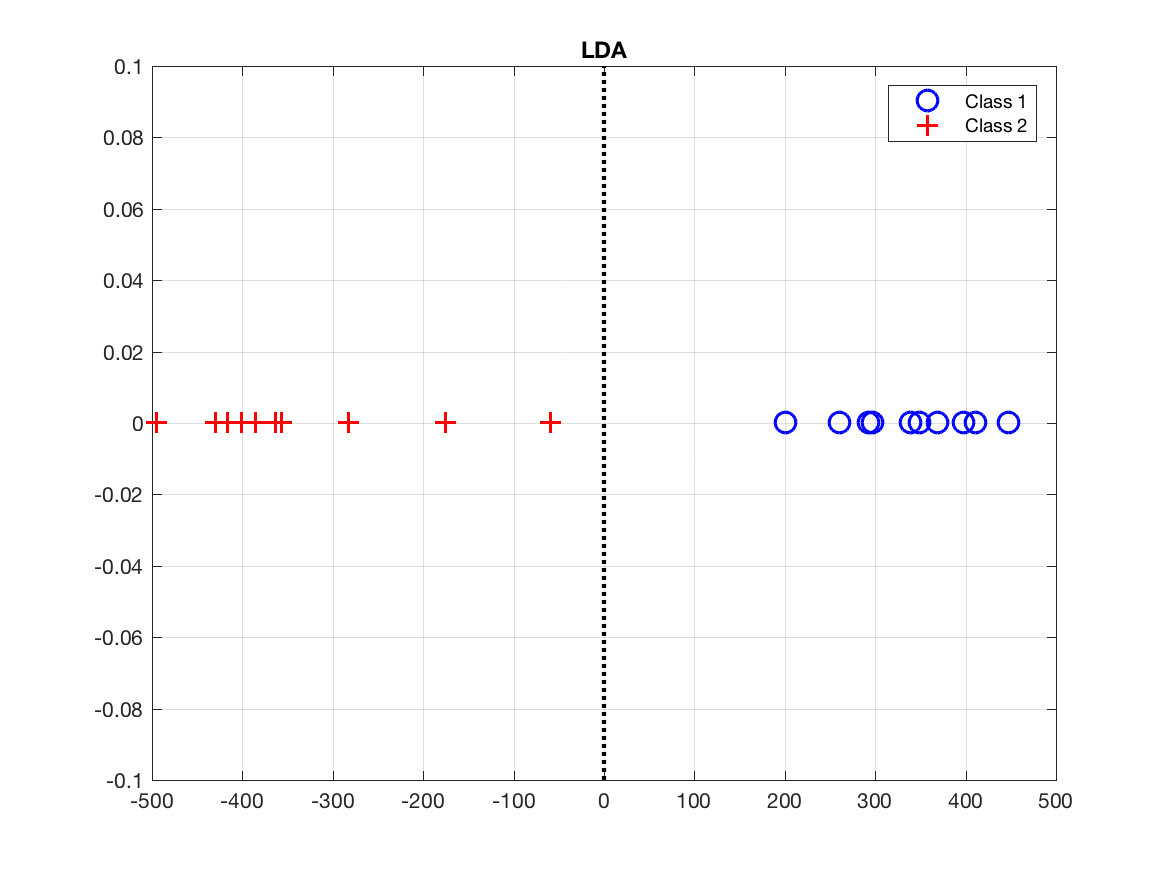
\includegraphics[trim={0cm 1cm 0cm 0cm},clip,width=0.60\columnwidth]{../data/classify_KL}
        \caption{LDA using SVD on the mean-subtracted data}
        \label{fig:lda_2}
        \end{figure}
    \end{minipage}
}

\end{homeworkSection}

\newpage
\begin{homeworkSection}{3. Maximum Noise Fraction (MNF) method}
Construct a $n \times 10$ matrix (choose $n \geq 250$) to serve as a ground truth data set so that each column is a
$n$-dimensional time series. Next, add \textbf{correlated noise} to each column to create a noisy data set, $X$. The
goal of this problem is to implement the Maximum Noise Fraction method to recover the ground truth as
closely as possible from the noisy data. Suppose the source of the noise is unknown, you may estimate
the noise covariance, $N^TN$, using the difference matrix as $N^T N = \frac{1}{2} dX^TdX$ where if
$$
    X = \begin{bmatrix}
        x_1(t_1)  &&  x_2(t_1) && \cdots && x_p(t_1) \\
        x_1(t_2)  &&  x_2(t_2) && \cdots && x_p(t_2) \\
        \vdots    && \vdots    && \ddots && \vdots \\
        x_1(t_n)  &&  x_2(t_n) && \cdots && x_p(t_n)
    \end{bmatrix}
$$
then
$$
    dX = \begin{bmatrix}
        x_1(t_2)-x_1(t_1)  &&  x_2(t_2)-x_2(t_1) && \cdots && x_2(t_2) - x_p(t_1) \\
        x_1(t_3)-x_1(t_2)  &&  x_2(t_3)-x_2(t_2) && \cdots && x_2(t_3) - x_p(t_2) \\
        \vdots    && \vdots    && \ddots && \vdots \\
        x_1(t_n)-x_1(t_{n-1})  &&  x_2(t_n)-x_2(t_{n-1}) && \cdots && x_2(t_n) - x_p(t_{n-1})
    \end{bmatrix}
$$
Notice that $X \in \mathbb{R}^{n \times p}$ and $dX \in \mathbb{R}^{(n-1) \times p}$.
In your report, examine and elaborate on the effect of a $D$-mode
reconstruction on a single noisy signal for various values of $D$ (i.e., choose a single column to filter). In a single graph, visually display the result of the original signal, noisy signal, and filtered (de-noised) data
(with your best choice of $D$) to compare. Use the graph legend to distinguish each.
\\
\\
\problemAnswer{
    According to \cite{kirby}, the MNF optimal basis is found via:
    \begin{itemize}
    \itemsep0em
    \item Take the eigenvector expansion of the covariance of $dX^T dX = V_1 \Sigma_1^2 V_1^T$.
    \item Whiten the original data: $\hat{X} = X V_1 \Sigma_1^{-1}$.
    \item Use the eigenvector expansion of the covariance of $\hat{X}$: $\hat{X}^T \hat{X} = U_1 \Sigma _2^2 U_1^T$.
    \item Define $\Psi = V_1 \Sigma_1^{-1} U_1^T$.
    \item Compute the maximum noise fraction basis vectors via $\Phi = X \Psi$.
    \end{itemize}

    Then our signal $S = \Phi$. Unfortunately, I was not able to effectively produce desired results, as seen in Figure \ref{fig:mnf}.

    \begin{minipage}{1.0\textwidth}
        \begin{figure}[H]
        \centering
        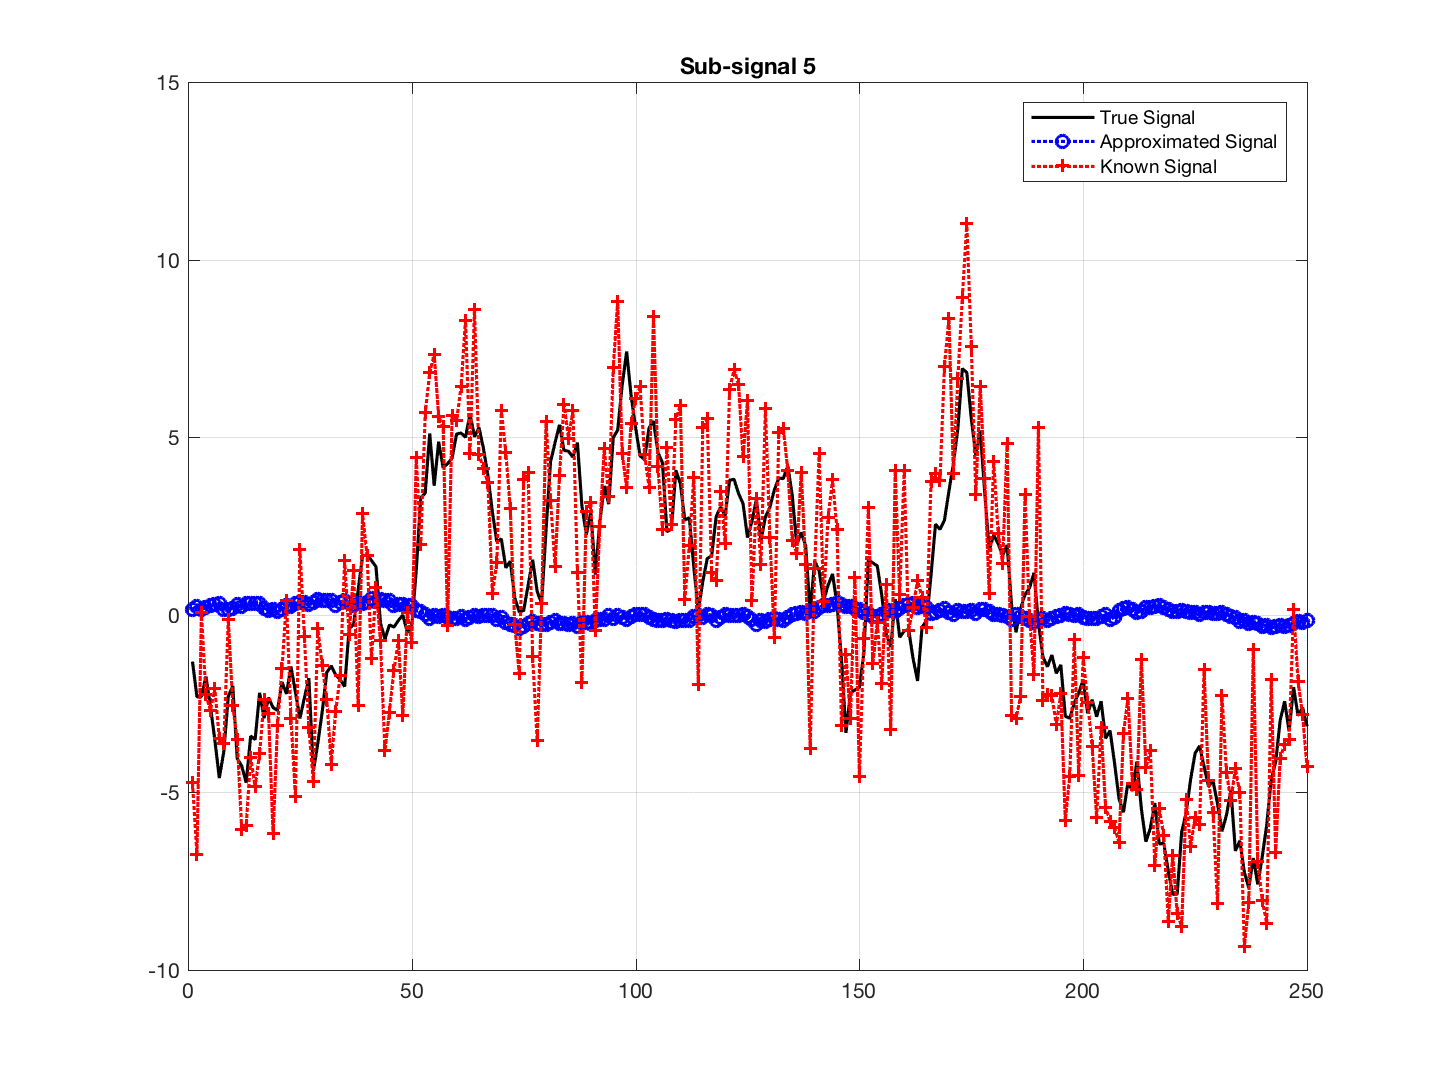
\includegraphics[trim={0cm 1cm 0cm 1cm},clip,width=0.60\columnwidth]{../data/MNF}
        \caption{MNF for noise elimination}
        \label{fig:mnf}
        \end{figure}
    \end{minipage}
}

\end{homeworkSection}

\end{section}
%----------------------------------------------------------------------------------------

\appendix

\section{Code}\label{code}

\subsection{KL Procedure for Gappy Data}
\lstinputlisting{../repair_gappy_data.m}

\subsection{LDA}
\lstinputlisting{../LDA.m}

\subsection{MNF}
\lstinputlisting{../MNF.m}


\begin{thebibliography}{10}
    \bibitem{chang}
    Chang, Jen-Mei. \textit{Matrix Methods for Geometric Data Analysis and Recognition}. 2014.

    \bibitem{fisher}
    P. N. Belhumeur, J. P. Hespanha and D. J. Kriegman, ``Eigenfaces vs. Fisherfaces: recognition using class specific linear projection," in \textit{IEEE Transactions on Pattern Analysis and Machine Intelligence}, vol. 19, no. 7, pp. 711-720, Jul 1997.

    \bibitem{everson}
    R. Everson and L. Sirovich. The karhunen-loeve transform for incomplete data. \textit{J. Opt. Soc. Am., A}, 12(8):1657–1664, 1995.

    \bibitem{kirby}
    Hundley, D., Kirby, M., and Anderle, M. \textit{A SOLUTION PROCEDURE FOR BLIND SIGNAL SEPARATION USING THE MAXIMUM NOISE FRACTION APPROACH: ALGORITHMS AND EXAMPLES}.
    <https://inc.ucsd.edu/ica2001/115-hundley.pdf>.

    \bibitem{debbie}
    Tonne, Debbie. Helped with emphasizing dimensionality reduction before doing LDA.
\end{thebibliography}

\end{document}
